\documentclass[11pt]{article}
\usepackage[T1]{fontenc}
\usepackage{lmodern}
\usepackage[margin=0.9in]{geometry}
\usepackage{amsmath,amssymb,amsthm}
\usepackage{graphicx}
\usepackage{booktabs}
\usepackage[font=small,labelfont=bf]{caption}
\usepackage[hidelinks]{hyperref}
\usepackage{float}
\graphicspath{{../figures/}}

\theoremstyle{definition}
\newtheorem{definition}{Definition}[section]
\newtheorem{remark}[definition]{Remark}

\title{\textbf{Is Your Girlfriend a Spy?}\\[4pt] \large A base-rate analysis of honey traps, from regular people all the way up to the CEO's family}
\author{Django Thompson}
\date{12 November 2026}

\raggedbottom
\begin{document}
\maketitle

\begin{abstract}
\noindent
Is your girlfriend a spy? Using FBI, Census and security clearance data, I find that for a normal person it's about 1 in 8.5 million, seven times less likely than getting hit by lightning this year. As expected, it climbs fast the closer you are to power: 1 in 13{,}100 with Top Secret clearance, 1 in 333 if you're a CEO family member, 1 in 100 if you're the CEO. Red flags barely matter if you're a nobody. They matter a lot if you're somebody's son.
\end{abstract}

\noindent{\small\textit{Disclaimer.} This is satirical. The spying claims about the Jensen Huang affair are unproven allegations, nobody has been charged, and nothing here says otherwise. Please don't go through your partner's phone. I used AI to help with the code and checking sources.}

\section{Why this exists}

This week, as we all know, Nvidia's CEO Jensen Huang admitted to an affair with a woman US officials reportedly believe is a Chinese spy~\cite{ap,tc}. Reports also claim she helped move about \$7.5 billion of Nvidia chips into China, some of them banned~\cite{tc}. Nvidia denies any wrongdoing, and none of the spying claims have been proven. Huang has resigned anyway, and Nvidia's stock fell more than 10\% in a week~\cite{tc,abc}. If the reports are right, he walked straight into a honey trap and is now paying for it. So naturally everyone is asking whether their own girlfriend is a secret government spy.

\begin{definition}[Spy girlfriend]
Your partner is a \emph{spy girlfriend} if, right now, the relationship is part of an active foreign intelligence operation aimed at you. Boyfriends count too. The trend just happened to pick girlfriends.
\end{definition}

\section{The model}

Nobody is running a honey trap on a random guy from Croydon. Romance takes months and ends up on the news if it goes wrong, so you save it for someone who actually has something worth stealing.

So the number that matters is how many romance operations there are and how many people they get shared between. For a group $g$ of $N_g$ people,
\begin{equation}
P(\text{spy} \mid g) \;=\; \frac{C \, \rho \, s_g}{N_g}.
\end{equation}
Here $C$ is the number of active counterintelligence cases and $\rho$ is the share that involve a relationship. $s_g$ is the share of those aimed at group $g$.

\paragraph{Real inputs.} FBI Director Christopher Wray said in July 2020 that the Bureau had ``nearly 5{,}000 active FBI counterintelligence cases'', roughly half tied to China~\cite{wray}. So $C = 5{,}000$. The US has 258.3 million adults~\cite{census}. The last public clearance count found 4.03 million people cleared for classified information, about 2.7 million at Confidential or Secret and 1.3 million at Top Secret~\cite{odni}. There are 500 Fortune 500 CEOs.

\paragraph{Guessed inputs.} I don't know $\rho$. Nobody outside the FBI does. I went with 5\%. I also had to guess how many people sit around each CEO. I went with about nine senior executives, five close family members (spouse, kids, parents) and two people who run the CEO's life, like an executive assistant or chief of staff. That gives 4{,}500 executives, 2{,}500 family members and 1{,}000 assistants. The romance cases get split 12\% regular people, 36\% Secret, 40\% Top Secret, 4\% executives, 3\% family, 3\% assistants and 2\% CEOs. All of this gets shaken around in Section~\ref{sec:sens}.

\begin{remark}
One case isn't one spy. Some cases have several people in them, loads are tips that go nowhere, and most are about hacking or stolen tech. That's why $\rho$ is small. It also means the numbers here are probably too high for most of you, which is good news.
\end{remark}

\section{Results}

\begin{table}[H]
\centering\small
\begin{tabular}{lrrr}
\toprule
Who you are & People & Point estimate & 90\% interval \\
\midrule
Regular adult & 254 million & 1 in 8.5 million & 1 in 69M to 1 in 1.6M \\
Secret clearance & 2.7 million & 1 in 30{,}000 & 1 in 154{,}000 to 1 in 6{,}200 \\
Top Secret clearance & 1.3 million & 1 in 13{,}100 & 1 in 65{,}000 to 1 in 2{,}700 \\
Fortune 500 senior exec & 4{,}500 & 1 in 450 & 1 in 21{,}000 to 1 in 69 \\
Close family of a CEO & 2{,}500 & 1 in 333 & 1 in 42{,}000 to 1 in 49 \\
CEO's assistant or chief of staff & 1{,}000 & 1 in 133 & 1 in 17{,}000 to 1 in 20 \\
Fortune 500 CEO & 500 & 1 in 100 & 1 in 105{,}000 to 1 in 14 \\
\bottomrule
\end{tabular}
\caption{Chance your partner is currently working a case on you. Intervals come from the simulation in Section~\ref{sec:sens}.}
\end{table}

\subsection{If you are a normal person}

You're fine. Getting hit by lightning this year is seven times more likely (1 in 1.2 million~\cite{nws}). Pulling the Pirate Shop Token out of one Fortnite chest is 62 times more likely (1 in 137{,}500~\cite{epic}). Your girlfriend asking why you liked that person's post is the closest you'll ever get to an interrogation.

\subsection{If you are close to someone important}

A CEO's kid doesn't have a clearance or sign anything, but they live in the same house as someone who does. They hear the phone calls, use the home Wi-Fi and know where the laptop lives. Nobody ever trained them to be suspicious, so they're a much easier target than the CEO, who has a security team and a lawyer on speed dial.

You can see it in Figure~\ref{fig:ladder}. Family sits right next to the CEO, and the assistant is basically level with the boss. The person booking the flights sees the calendar, and the calendar is usually what's worth stealing. By my numbers, being a CEO's son is about 25{,}000 times riskier, romantically, than being a normal son. Tough luck, rich kids.

\subsection{If you are the CEO}

About 1 in 100. Sounds terrifying until you see the interval, which runs from 1 in 14 to 1 in 105{,}000. There are only 500 of them, so one extra operation swings it massively. Don't quote this one without the range.

I did not work out a separate number for Jensen. The sample size is one, and his lawyers outnumber it. What I can say is that he wasn't an average Fortune 500 CEO. Before this week Nvidia was the second most valuable company in the world, at about \$4.2 trillion, behind only Apple~\cite{cmc}. Pretty much every country relies on its chips to build AI. He also did almost every product launch in the same black leather jacket, so he's not exactly hard to spot in a crowd. By the logic of this model, that puts him about as far right on Figure~\ref{fig:ladder} as a person can go.

\begin{figure}[H]
\centering
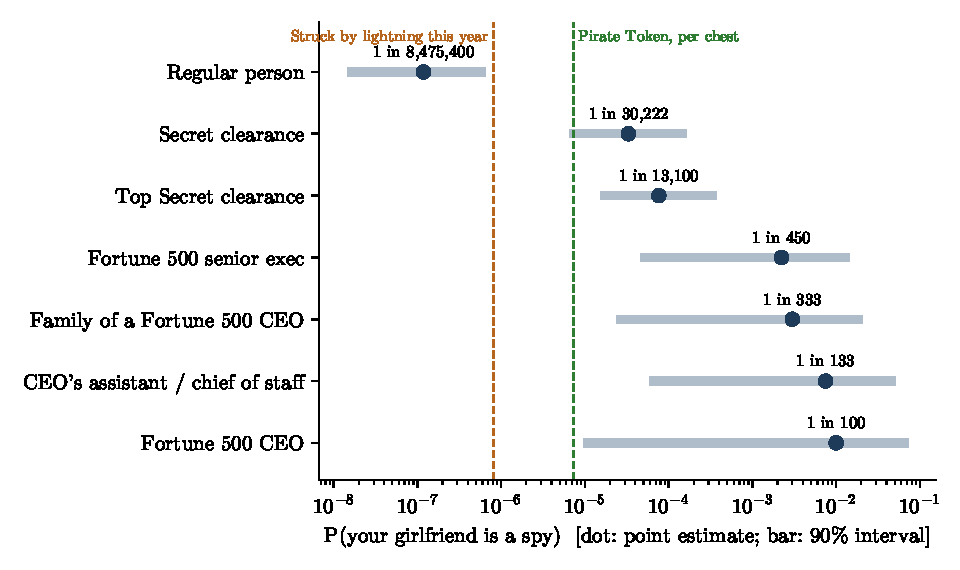
\includegraphics[width=\linewidth]{fig_ladder.pdf}
\caption{The access ladder. The closer you are to something worth stealing, the further right you go. Both dashed lines are also things that will not happen to you.}
\label{fig:ladder}
\end{figure}

\section{But she has red flags}

A red flag only counts as evidence if spies do it way more than normal people do. That ratio is called the likelihood ratio (LR). You start from your odds in Table~1 and multiply by each flag's LR. I'm pretending the flags are independent. In reality, they aren't, so this is being generous.

\begin{table}[H]
\centering\small
\begin{tabular}{rlr}
\toprule
\# & Red flag & Assumed LR \\
\midrule
1 & Asks what you do at work & 1.05 \\
2 & Uses a VPN & 1.3 \\
3 & Is ``mysterious'' & 1.2 \\
4 & Has two phones & 3 \\
5 & Very interested in your (or your dad's) security clearance & 25 \\
6 & Asked for your laptop password on the first date & 40 \\
\bottomrule
\end{tabular}
\caption{Every LR here is made up. Focus on the pattern rather than the decimals. Most people do flags 1 to 3.}
\end{table}

For a normal person, flags 1 to 3 take you from 1 in 8.5 million to 1 in 5.2 million. So ``she's mysterious and uses a VPN'' is worth basically nothing. Tick all six and you get to 1 in 1{,}700, which means she's still almost certainly not a spy, just a bit weird.

Higher up, the same six flags do real damage (Figure~\ref{fig:flags}). Top Secret clearance ends up at 27\%. A CEO's family member goes past 90\%, from exactly the same evidence, because they started so much higher up.

People always ask about where she's from. I left that out on purpose. Millions of people from every country live in the UK and the US, and nearly all of them are not spies, so passports barely move the odds. The only thing that actually affects your probability is whether you're close to someone actually important and worth spying on. It's not her passport. It's your dad's job.

\begin{figure}[H]
\centering
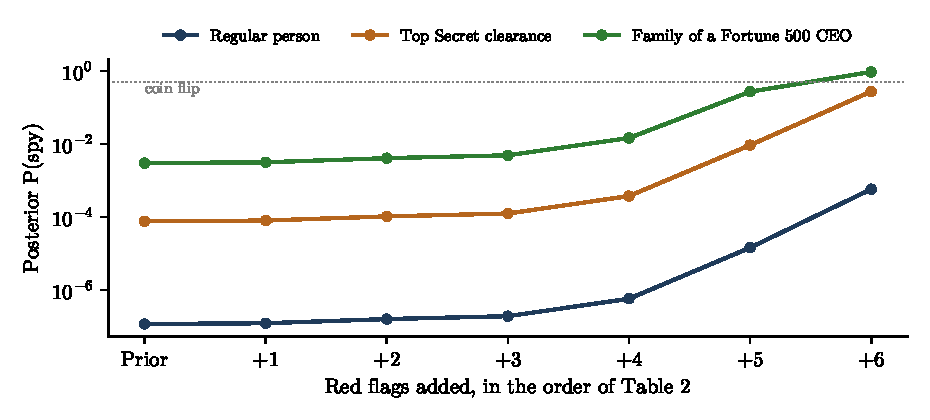
\includegraphics[width=\linewidth]{fig_flags.pdf}
\caption{Identical red flags. A regular person never gets near the coin-flip line. A CEO's family member crosses it.}
\label{fig:flags}
\end{figure}

People make this mistake so often it has a name, base-rate neglect~\cite{kahneman}. Something that sounds suspicious feels like proof, but when the thing you're looking for is one in millions, almost everyone who gets flagged is innocent. Doctors have the exact same problem with screening tests~\cite{gigerenzer}.

\section{Sensitivity}\label{sec:sens}

Because half my inputs are guesses, I reran everything 100{,}000 times. The case count $C$ ranged from 2{,}500 to 10{,}000, because cases aren't people and Wray's number is six years old. The romance share $\rho$ ran from 1\% to 20\% on a log scale, and the group split moved around my guesses using a Dirichlet distribution. The intervals in Table~1 are the 5th and 95th percentiles.

A few results barely moved. In 95\% of runs a regular adult stayed below 1 in 1.6 million. In every run, a Secret clearance was at least 10 times riskier than having none, and the typical gap was about 300 times. A CEO's close family came out ahead of Top Secret clearance holders in 91\% of runs. The order inside the inner circle (exec, family, assistant, CEO) is the shakiest part, since those groups are small and their shares are pure guesses.

\section{Limitations}

How the romance cases split across groups is invented. So are the sizes of each CEO's inner circle. The FBI count covers the US only, dates from 2020, and lumps every country together. I treat the relationship as a snapshot, so anyone in a long relationship has a slightly higher lifetime chance than shown. People recruited partway through a relationship aren't modelled, though that does happen~\cite{csis}. I also assume spies only date people for access, which is maybe a bit harsh on spies.

\section{Conclusion}

If you're reading this, I can almost guarantee you're fine, as you clearly have too much spare time to be important enough to be spied on. It only changes once you're close to real power. CEOs at least have security teams. Their kids, partners and assistants mostly don't, and in this model they're nearly as exposed. So if your mum runs a Fortune 500 company and your new girlfriend keeps asking about her diary, maybe worry a bit. The chance that snooping ends your relationship is a lot higher than 1 in 8.5 million.

\begin{thebibliography}{9}\small
\bibitem{ap} Associated Press. ``Nvidia CEO Jensen Huang resigns after his affair raises national security concerns.'' Via \textit{The Boston Globe}, 12 November 2026. Summarising reporting by \textit{The New York Times}; AP notes it could not independently confirm the reports.
\bibitem{tc} Silberling, A. ``The unfolding Jensen Huang scandal: a timeline.'' \textit{TechCrunch}, 12 November 2026. The \$7.5 billion figure is from \textit{The Information}, citing unnamed sources.
\bibitem{abc} Zahn, M. ``Nvidia closes lower after CEO Jensen Huang resigns.'' \textit{ABC News}, 12 November 2026.
\bibitem{cmc} CompaniesMarketCap. ``NVIDIA (NVDA) market capitalization.'' \$4.195 trillion at close on 11 November 2026, ranked 2nd worldwide. Accessed 12 November 2026.
\bibitem{wray} Wray, C. ``The threat posed by the Chinese government and the Chinese Communist Party to the economic and national security of the United States.'' Remarks at the Hudson Institute, Washington DC, 7 July 2020.
\bibitem{census} U.S. Census Bureau. ``2020 Census: adult population (18 and over) of 258.3 million.'' 2021.
\bibitem{odni} Office of the Director of National Intelligence. \textit{Fiscal Year 2017 Annual Report on Security Clearance Determinations}, Table 1.3 (total eligible as of 1 October 2017). 2018.
\bibitem{nws} National Weather Service. ``How dangerous is lightning?'' Odds of being struck in a given year: 1 in 1{,}222{,}000.
\bibitem{epic} Epic Games. Fortnite Pirate Shop Token drop rate, 1 in 137{,}500 chests. November 2026. See also Thompson, D. ``Token or True Love?'' Zenodo, 2026.
\bibitem{kahneman} Kahneman, D. and Tversky, A. ``On the psychology of prediction.'' \textit{Psychological Review} 80(4):237--251, 1973.
\bibitem{gigerenzer} Gigerenzer, G. et al. ``Helping doctors and patients make sense of health statistics.'' \textit{Psychological Science in the Public Interest} 8(2):53--96, 2007.
\bibitem{csis} Center for Strategic and International Studies. ``Survey of Chinese espionage in the United States since 2000.'' Continuously updated.
\end{thebibliography}

\end{document}
